\section{Exploratory data analytics}

\subsection{Variables and frequency}
A \textit{variable} is any characteristic whose value may change from one observation to another. Making observations on variables results in data, which can be classified as:
\begin{itemize}
	\item Univariate dataset, with a single variable;
	\item Bivariate dataset, with two variables;
	\item Multivariate dataset, with two or more variables.
\end{itemize}

Data are called categorical, qualitative or nominal if the individual observations belong in one of several possible groups.

Categorical data are ordinal if those groups can be ordered (from the biggest to the smallest).

Data are numerical, quantitative or metric if the individual observations are real-valued numbers where numerical operations can be performed: they are classified in discrete and continue.

À frequency distribution for categorical data displays the possible categories along with their frequency or relative frequencies (number of times the category appears in the dataset). The relative frequency is the proportion between a frequency and the total observations.

The cumulative frequency table displays the proportion of values falling below the upper end of each interval, calculated summing the previous relative frequencies with the current one.

\subsection{Charts}
A bar chart is a graph of bars, with heights equal to either the frequencies or the relative frequencies. Its analog for continuous data (usually grouped in intervals)is the histogram.

\begin{figure}[h]
	\centering
	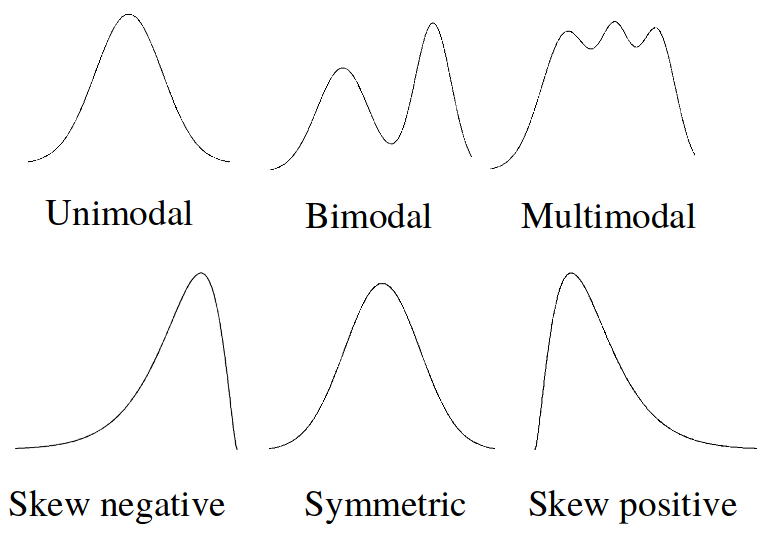
\includegraphics[scale=0.4]{lectures/images/distribution-shapes.png}
\end{figure}

A pie chart uses the familiar notion of a slice of pie to compare variable frequencies.

The dotplot is an alternative to the barplot used with continuous or discrete numerical data, showing each of the values along with their location. It is useful to highlight the most common values with their spread and outliers, allowing quick comparisons between categorical groups.

Steam and leaf plots work well with small datasets, showing consecutively increasing stems and one leaf for each number with the same stem.

\subsection{Medians, quartiles}
Those values can be obtained after a preprocessing, ordering the $n$ observations from smallest to largest:
\begin{itemize}
	\item Median:
	\begin{itemize}
		\item If $n$ is odd, the middle value;
		\item If $n$ is even, the mean of the two middle values;
	\end{itemize}
	\item Lower quartile, median of the lower half of the data;
	\item Upper quartile, median of the upper half of the data;
	\item Interquartile range (iqr), calculated as the difference between upper and lower quartile.
\end{itemize}

If an observation is more than 1.5 iqr away from the closest end of the interval, it is defined an outlier. An outlier is extreme if it falls further than 3 iqr, otherwise mild. 

A boxplot represents outliers with shaded or open circles, according to their type, and whiskers extending toward observations which are not outliers.

\section{Mean and variance}
The sample mean is calculated as:
$$\bar{x} = \frac{x_1 + x_2 + \dots + x_n }{n} = \frac{\sum x}{n}$$
It doesn't always consist in an accurate representation of the dataset: it can be broadly affected by outliers. Visualising the data is useful for a deeper insight.

Outliers can be removed since they have a great impact while not being descriptive of the data. The trimmed mean is the mean of a subset of the ordered values, excluding the extreme ones (trimming percentage).

The range identifies variability of data, using the difference between the largest and smallest value. This is defined deviation, and it is summarized using sample variance and standard deviation.
$$s^2 = \frac{(x - \bar{x})^2}{n - 1}$$
$$s = \sqrt{s^2} = \sqrt{\frac{(x - \bar{x})^2}{n - 1}}$$
$s^2 \geq 0$ and becomes larger as data becomes further from the mean. Outliers have an extreme impact on variance and standard deviation.

The standardization operation allows to extract $Z$-score from data, explaining how many standard deviations the observation is far from the mean:
$$Z = \frac{x_i - \bar{x}}{s}$$

\section{Bivariate data}
When data depends on two dimensions, it can be represented using a scatterplot. Points within the two axes might have a linear relationship, named correlation and calculated with the Pearson coefficient:
$$r = \frac{1}{n-1} \sum \Big( \frac{x - \bar{x}}{s_x} \Big) \Big( \frac{y - \bar{y}}{s_y} \Big)$$
Properties of $r$:
\begin{itemize}
	\item Does not depend on unit of measurement or axis selection;
	\item Always between +1 and -1;
	\item Not appropriate for non-linear relationships.
\end{itemize}
\begin{figure}[h]
	\centering
	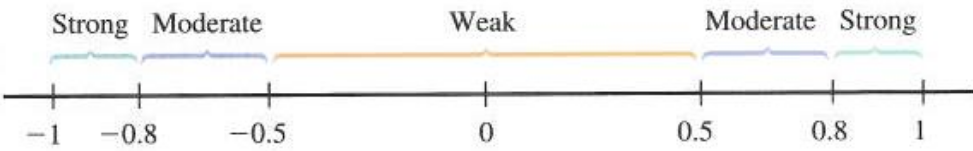
\includegraphics[scale=0.5]{lectures/images/r.png}
\end{figure}
A linear relation has equation of $y = a = bx$ where $b$ is the slope and $a$ is the intercept. A measure for the goodness of fit of a line to bivariate data is the least squares criterion, using the vertical distance:
$$\sum \big[ y - (a + bx)^2 \big]$$
The smallest distance is found setting the partial derivatives to 0 and solving the equation.

Steps in linear regression:
\begin{enumerate}
	\item Determining the explanatory and response variable;
	\item Looking at the scatterplot to find any potential linear relationship;
	\item Checking for unusual patterns;
	\item Observing predictions and their accuracy.
\end{enumerate}
The predicted or fitted values result from substituting each sample $x$ value into the equation for the least squares line.

Residuals are the values $y_1 - \hat{y}_1, \dots, y_n - \hat{y}_n$, and correspond to the vertical difference. Plotting those results can be explicative for potential problems or under-prediction.

Another indicator consists in the total sum of squares $\sum (y - \bar{y})^2$ and measures the distance from the horizontal line.

Coefficient of determination:
$$r^2 = 1 - \frac{\sum y^2 - \frac{(\sum y)^2}{n}}{\sum y^2 - a\sum y - b \sum xy} = \frac{\text{total sum of squares}}{\text{reidual sum of squares}}$$
It ranges between 0 and 1, higher values represent a better prediction. $r^2$ is the percent of variation in $y$ that can be explained by $x$.

The standard deviation about the least squares line is denoted $s_e$ and interpreted as the typical amount by which an observation deviates from the least squares line.
$$s_e = \sqrt{\frac{\text{SSResid}}{n - 2}}$$

If the scatterplot does not look linear, it is possible to apply transformations to the variables (such as logarithm) to obtain a better fit.

Since observations occurring over time are not often independent, using a time series plot with time on the x-axis can be uninformative.

